\documentclass[11pt]{article}
\usepackage[margin=1in]{geometry}
\usepackage[T1]{fontenc}
\usepackage[utf8]{inputenc}
\usepackage{lmodern}
\usepackage{amsmath,amssymb,booktabs}
\usepackage{graphicx}
\usepackage{microtype}
\IfFileExists{xurl.sty}{\usepackage{xurl}}{\usepackage[hyphens]{url}}
\setlength{\emergencystretch}{3em}

\title{Fertility, Baby Booms, and the Political Economy of Housing Supply}
\author{Draft for project 03\\(extension of the NIMBY housing-supply model)}
\date{March 1, 2026}

\begin{document}
\maketitle

\begin{abstract}
This paper develops a fertility extension of the NIMBY housing-supply framework from project 02.
The baseline project-02 mechanism links local political preferences to endogenous housing supply
tightness. The extension adds endogenous fertility and a lagged cohort-political channel:
a temporary baby-boom shock can increase later political resistance to housing supply, raise
future housing prices, and reduce later fertility. We present side-by-side simulations against
an old-model proxy that excludes the fertility channel, and we clarify exactly what the current
prototype can and cannot establish. The model is a mechanism exercise and does not yet identify
causal effects in US data. We close with an empirical implementation plan for a US fertility
panel with explicit immigration/cohort accounting.
\end{abstract}

\section{Introduction}

The main question is whether demographic shocks can feed back into housing politics and then
affect fertility in the next generation. In the original NIMBY model, housing supply outcomes are
determined by political equilibrium and demand pressures. In this extension, fertility and
demographics are no longer exogenous background objects: they are part of the state transition.

The conceptual sequence is:
\begin{enumerate}
\item A baby-boom shock temporarily raises births.
\item As these cohorts age into politically relevant groups, local supply preferences tighten.
\item Tighter supply raises housing costs and can lower subsequent fertility.
\end{enumerate}

This paper is intentionally separate from project 02. It reuses the political housing-supply core,
but asks a distinct question and introduces new dynamic channels.

\section{Relation to the NIMBY paper}

Table \ref{tab:crosswalk} summarizes what is inherited from project 02 and what is new here.

\begin{table}[h!]
\centering
\caption{Model crosswalk: project 02 versus project 03}
\label{tab:crosswalk}
\begin{tabular}{p{0.28\textwidth}p{0.33\textwidth}p{0.33\textwidth}}
\toprule
Component & Project 02 (NIMBY paper) & Project 03 (this paper) \\
\midrule
Political housing-supply block & Core mechanism & Inherited \\
Housing price dynamics & Endogenous & Inherited \\
Fertility choice & Exogenous / absent & Endogenous in new model \\
Demographic feedback to politics & Limited / exogenous demographics & Explicit lagged baby-boom cohort channel \\
Main experiment & Housing-policy and demand shocks & Temporary baby-boom shock plus fertility channel \\
Empirical target & Housing outcomes and political economy & Fertility dynamics plus housing politics \\
\bottomrule
\end{tabular}
\end{table}

\section{Model}

\subsection{Environment}

Time is discrete. The state includes age-distribution mass $M_t(j)$, housing price index $p_t$,
political tightness $\theta_t$, and lagged births that proxy children-at-home demand pressure.

Households in fertile-age bins choose fertility subject to housing costs. Housing supply depends
on political tightness and prices, as in the project-02 logic.

\subsection{Fertility block (new channel)}

Desired fertility rate:
\[
f_t^* = \text{clip}\left(f_{level}\exp(-\eta_p p_t),\,0.05,\,0.85\right).
\]

Observed births with a temporary baby-boom multiplier $\mu_t$:
\[
b_t = f_t^* \cdot \sum_{j \in \mathcal{F}} M_t(j) \cdot \mu_t,\qquad
\mu_t =
\begin{cases}
1+\text{boom\_amp}, & t \in [t_{start}, t_{end}]\\
1, & \text{otherwise}.
\end{cases}
\]

\subsection{Political tightness}

\[
\theta_t = \text{clip}\Big(
\theta_0
 + \theta_{old}\cdot old_t
 - \theta_{young}\cdot young_t
 + \theta_{boom}\cdot \overline{b}_{t-\ell:t-\ell-w+1},\;
0,\;0.95
\Big),
\]
where the lagged births term captures entry of baby-boom cohorts into politically relevant
homeowner/voter groups.

\subsection{Housing market update}

Demand:
\[
D_t = d_0 + d_{young}\cdot young_t + d_{birth}\cdot b_t + 0.15\cdot n^{home}_t.
\]

Supply:
\[
S_t = s_0 + \varepsilon_0(1-\theta_t)\exp(-p_t).
\]

Price law of motion:
\[
p_{t+1} = (1-\lambda)p_t + \lambda\left[p_t + g(D_t-S_t)\right].
\]

\section{Simulation design}

Baseline calibration (current prototype):
\begin{itemize}
\item Horizon $T=80$.
\item Damping $\lambda = 0.25$.
\item Baby-boom shock: +60\% births from $t=15$ to $t=24$.
\item Post-shock evaluation window starts at $t=40$.
\end{itemize}

We compare:
\begin{enumerate}
\item \textbf{New model}: endogenous fertility and lagged boom-to-politics channel.
\item \textbf{Old proxy}: pre-extension logic with no endogenous fertility response.
\end{enumerate}

\section{Side-by-side simulation results}

Figure \ref{fig:paths} and Figure \ref{fig:effects} provide dynamic paths and shock-minus-baseline
effects.

\begin{figure}[h!]
\centering
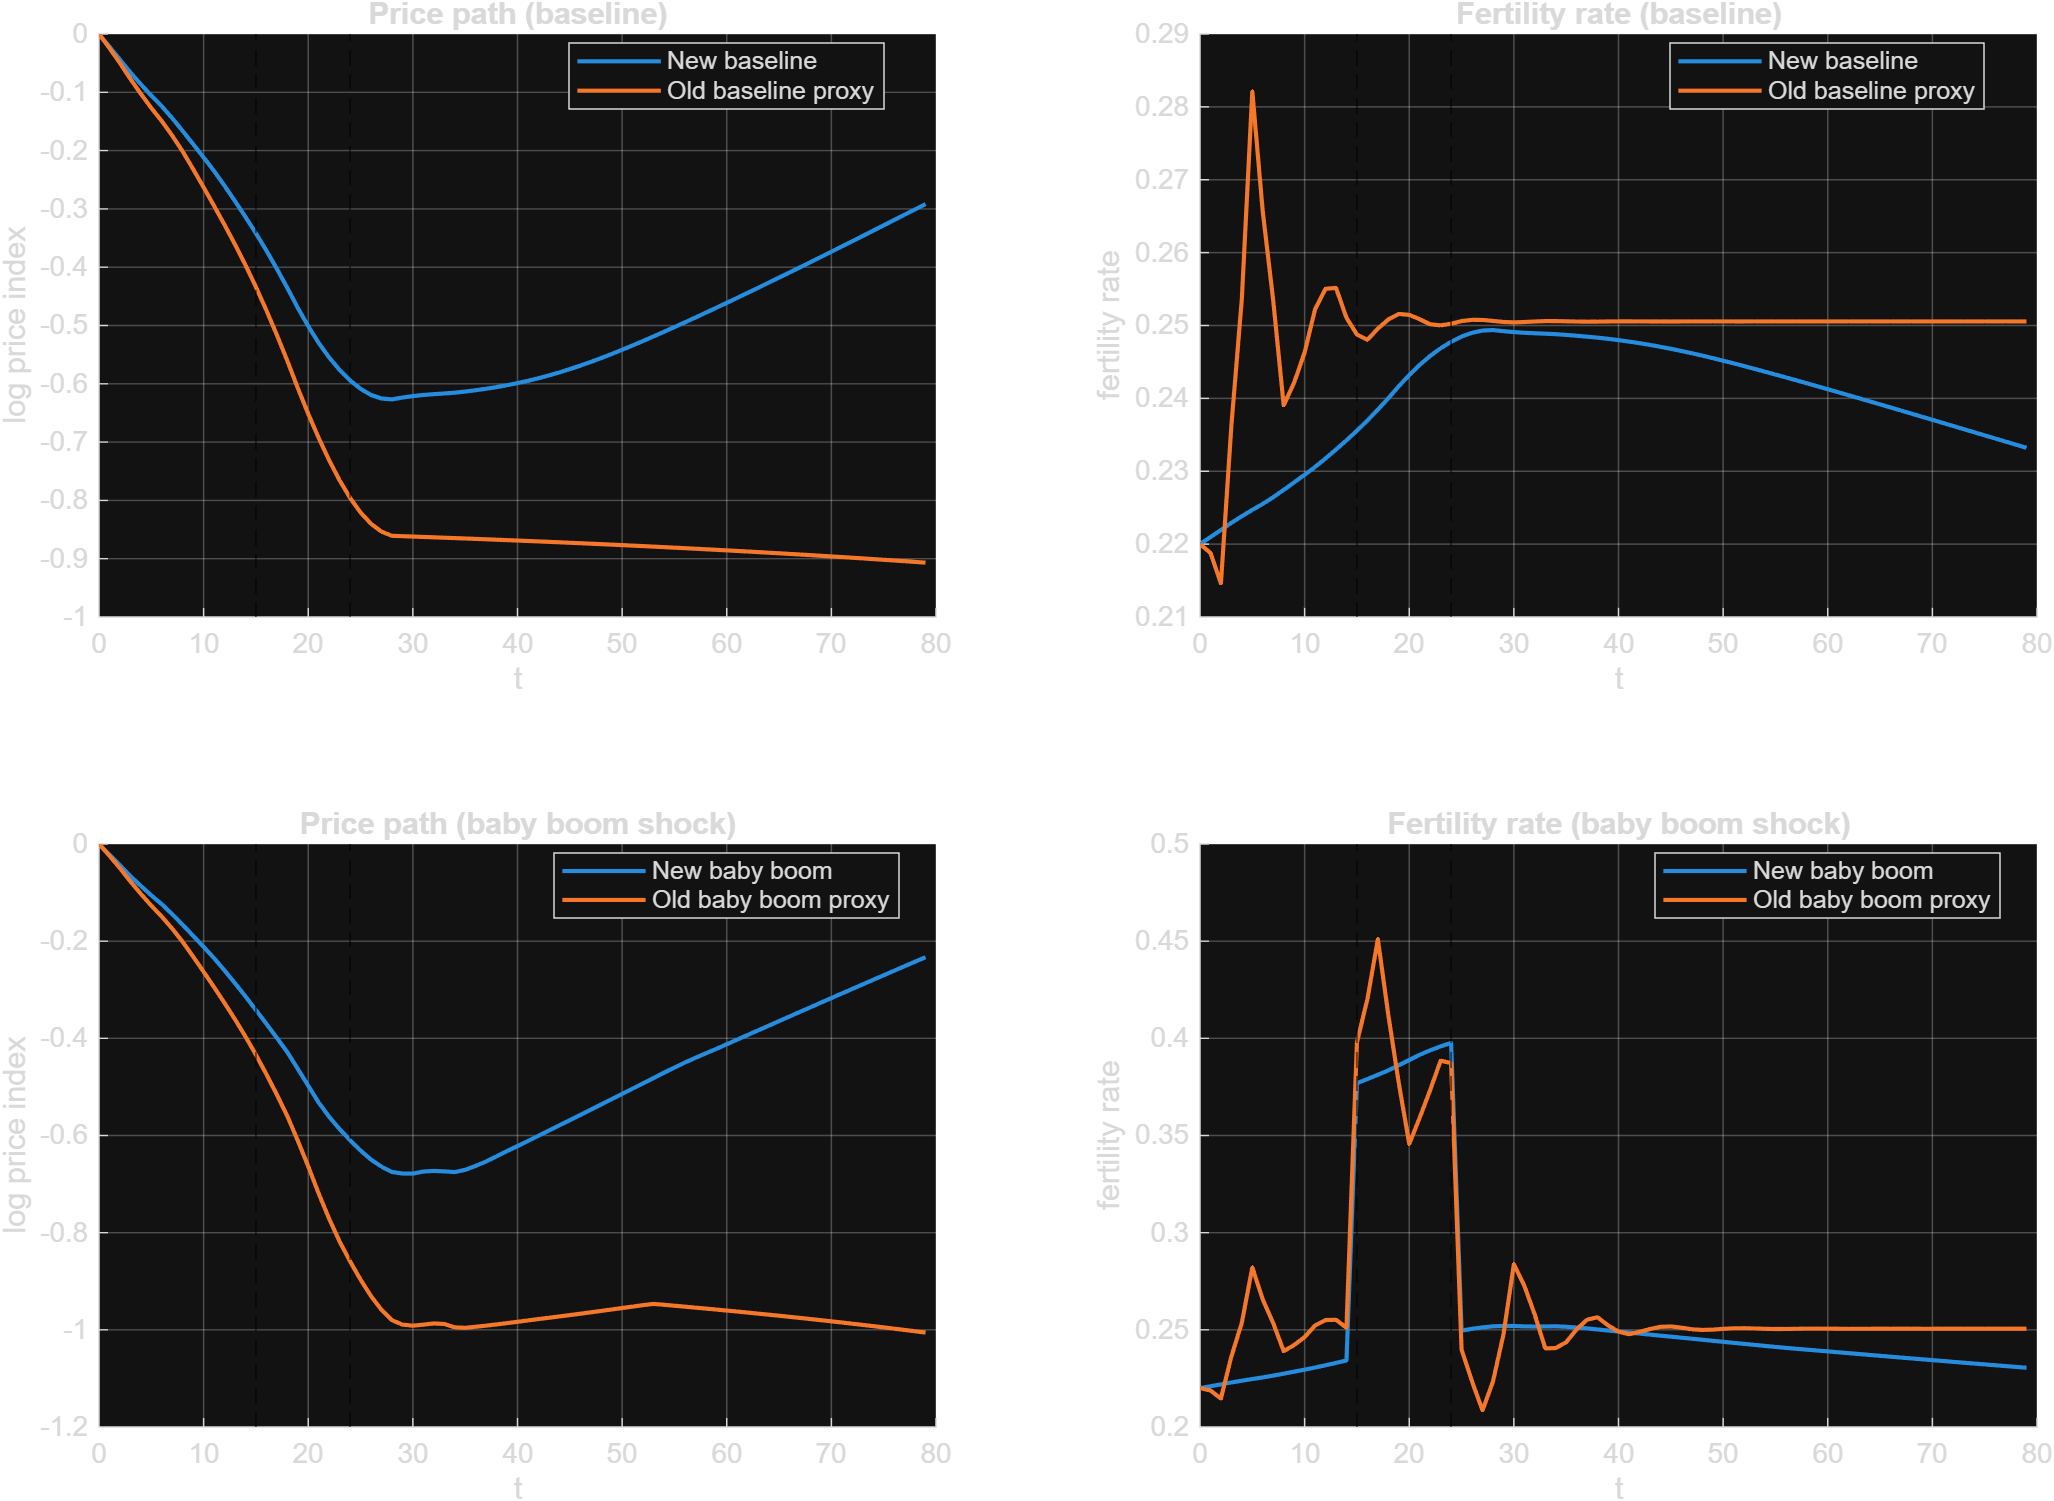
\includegraphics[width=0.92\textwidth]{../../../notes/build/old_vs_new_paths.png}
\caption{Baseline and shock paths, new model versus old proxy}
\label{fig:paths}
\end{figure}

\begin{figure}[h!]
\centering
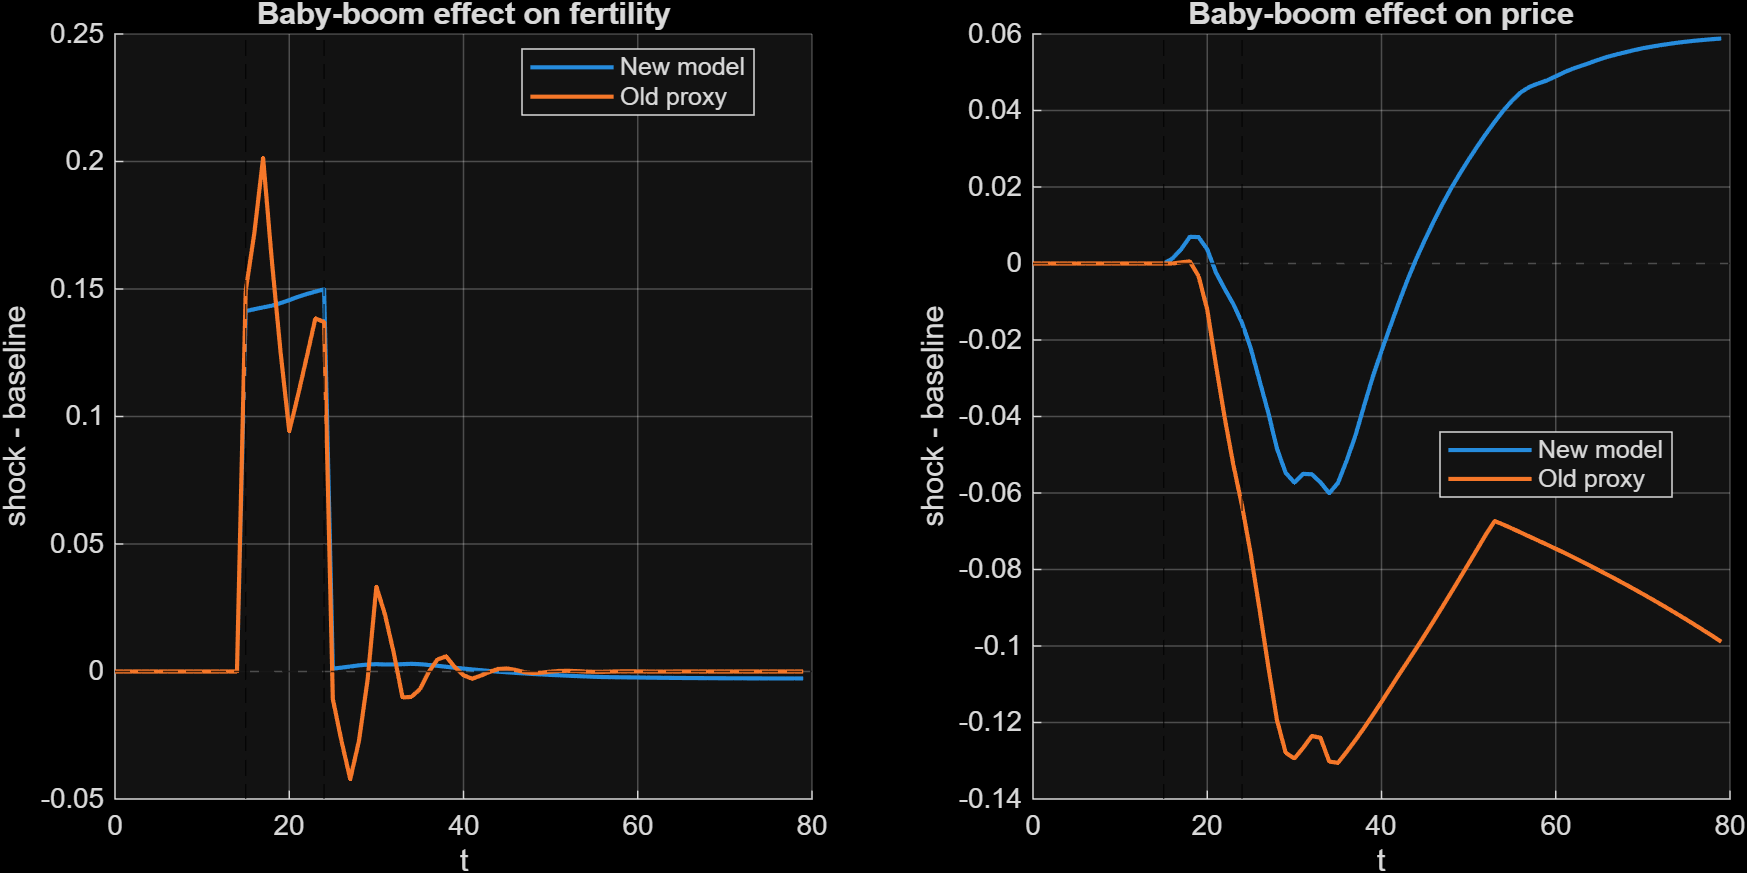
\includegraphics[width=0.92\textwidth]{../../../notes/build/old_vs_new_policy_effects.png}
\caption{Shock-minus-baseline effects on fertility and prices}
\label{fig:effects}
\end{figure}

Table \ref{tab:phase} summarizes the key phase deltas from the latest run.

\begin{table}[h!]
\centering
\caption{Phase deltas (shock minus baseline) from latest MATLAB run}
\label{tab:phase}
\begin{tabular}{lrrrrrr}
\toprule
Model & $\Delta f_{pre}$ & $\Delta f_{boom}$ & $\Delta f_{post}$ & $\Delta p_{pre}$ & $\Delta p_{boom}$ & $\Delta p_{post}$ \\
\midrule
New & 0.000000 & 0.145361 & -0.001812 & 0.000000 & -0.001259 & 0.038142 \\
Old proxy & 0.000000 & 0.141054 & -0.000107 & 0.000000 & -0.019750 & -0.085626 \\
\bottomrule
\end{tabular}
\end{table}

Interpretation:
\begin{enumerate}
\item During the boom window, fertility rises mechanically in both models.
\item In the new model, post-shock prices are higher and post-shock fertility is lower than baseline.
\item The old proxy does not deliver the same post-shock direction, highlighting the added channel.
\end{enumerate}

\section{What this does and does not show}

\subsection{What it shows}

The extension is internally consistent with the mechanism:
baby-boom cohorts can tighten later housing politics and modestly reduce later fertility,
conditional on calibration.

\subsection{What it does not show}

\begin{enumerate}
\item It does not yet establish a causal empirical effect in US data.
\item It is not yet the full project-02 steady-state stack; required upstream
      \texttt{.mat} inputs are not present in this repository copy.
\item Immigration and migration composition effects are not yet estimated empirically.
\end{enumerate}

\section{Empirical implementation: US fertility panel}

The immediate empirical objective is to test whether the model-implied dynamic pattern appears in
US data once migration/immigration composition is handled explicitly.

Panel target:
\begin{itemize}
\item Geography-time: county-year or MSA-year panel (state-year fallback).
\item Outcomes: age-specific fertility rates, first-birth timing proxies, cohort-completed fertility proxies.
\item Housing variables: permits, completions/unit mix, price/rent indices, reform timing.
\item Demographic controls: migration flows and foreign-born share changes by age cohort.
\end{itemize}

Identification:
\begin{enumerate}
\item Staggered event study around housing-supply reforms.
\item Political close-election design where feasible.
\item Geographic-supply IV as complementary margin.
\end{enumerate}

All baseline specifications will include immigration/cohort decomposition terms so that observed
fertility changes are not conflated with compositional shifts.

\section{Conclusion}

This paper is a separate project built on the NIMBY framework with one core extension:
endogenous fertility and lagged demographic-political feedback. The current model delivers
a plausible mechanism in which temporary baby booms can worsen later housing-supply politics
and reduce subsequent fertility. The next stage is empirical discipline using a US panel with
explicit immigration-aware cohort accounting.

\end{document}
